\chapter{Implementierung}
\section{Implementierung des Sprachverarbeitungssystems}\label{section:Implementierung_Sprachverarbeitung}
Um die Möglichkeit des Dialogs mit der Getränkmischmaschine zu realisieren, war es notwendig, ein Modell für das Dialogsystem zu implementieren. Das Projekt des Dialogsystems besteht aus den folgenden Komponenten:
\begin{itemize}
    \item train\_dialog\_model.py - der Code zum Einlesen der natürlichsprachlichen Daten in einen Trainingssatz und zur Verwendung eines sequenziellen neuronalen Netzes von Keras zur Erstellung eines Modells für die Klassifizierung.
    \item model\_classes.pkl - eine Liste verschiedener Klassen von Antworten.
    \item words\_for\_pattern.pkl - eine Liste verschiedener Wörter, die für die Mustererkennung verwendet werden können.
    \item patterns.json - ein Stapel von JavaScript-Objekten, die verschiedene Tags auflisten, die verschiedenen Arten von Wortmustern entsprechen.
    \item dialog\_model.h5 - das von train\_dialog\_model.py erstellte Modell.
\end{itemize}
Diese Komponenten wurden sowohl zur Erstellung eines Deep Learning Modells für Klassifizierung und zum Trainieren dieses Modells als auch zur Implementierung des Dialogsystems und Bafehlverarbeitungssystems verwendet.
\subsection{Implementierung des Klassifizierungsmodells}
Für die Implementierung des Modells wurden folgenden Python Bibliotheken und Klassen verwendet:
\begin{itemize}
    \item 'nltk': eine Python-Bibliothek für die Arbeit mit natürlichen Sprachdaten. Es bietet Werkzeuge für Aufgaben wie Tokenisierung, Stemming, Lemmatisierung, Part-of-Speech-Tagging und mehr.
    \item 'nltk('punkt')': die \ac{NLTK}-Daten, die für die Tokenisierung benötigt werden, bei der ein Text in einzelne Wörter zerlegt wird.
    \item 'nltk'('wordnet'): die \ac{NLTK}-Daten, die für die Lemmatisierung benötigt werden, d. h. die Reduzierung eines Wortes auf seine Grund- oder Wurzelform.
    \item 'json': Python-Bibliothek für die Arbeit mit \ac{JSON}-Daten, einem leichtgewichtigen Format für den Datenaustausch. Sie bietet Methoden zur Kodierung von Python-Objekten in das \ac{JSON}-Format und zur Dekodierung von \ac{JSON}-Daten in Python-Objekte.
    \item 'pickle': eine Python-Bibliothek zur Serialisierung und Deserialisierung von Python-Objekten. Sie kann verwendet werden, um ein Python-Objekt in einen Byte-Stream zu konvertieren, der in einer Datei gespeichert oder über ein Netzwerk übertragen und später wieder in ein Python-Objekt deserialisiert werden kann.
    \item 'numpy': eine Python-Bibliothek für numerische Berechnungen. Sie bietet Unterstützung für große, mehrdimensionale Arrays und Matrizen sowie eine große Sammlung mathematischer Funktionen, die mit diesen Arrays arbeiten.
    \item 'random': eine Python-Bibliothek zur Erzeugung von Zufallszahlen und zur Durchführung von Zufallsoperationen. Sie bietet Methoden zur Erzeugung zufälliger Ganzzahlen, zur Auswahl zufälliger Elemente aus einer Liste, zum zufälligen Mischen einer Liste und mehr.
    \item 'keras.models.Sequential': eine Klasse, die von der Keras-Bibliothek bereitgestellt wird, einer in Python geschriebenen \ac{API} für neuronale Netze auf hoher Ebene. Die Klasse Sequential wird verwendet, um einen linearen Stapel von Schichten für ein neuronales Netzwerkmodell zu erstellen.
    \item 'keras.layers.Dense': eine Klasse, die von der Keras-Bibliothek bereitgestellt wird, um eine vollständig verbundene neuronale Netzwerkschicht zu erstellen.
    \item 'keras.layers.Activation': eine von der Keras-Bibliothek bereitgestellte Klasse zur Anwendung von Aktivierungsfunktionen auf die Ausgabe einer Schicht eines neuronalen Netzes.
    \item 'keras.layers.Dropout': eine von der Keras-Bibliothek bereitgestellte Klasse zur Anwendung der Dropout-Regularisierung auf die Ausgabe einer neuronalen Netzwerkschicht.
    \item 'keras.optimizers.SGD': eine von der Keras-Bibliothek bereitgestellte Klasse zur Definition des stochastischen Gradientenabstiegs-Optimierers für das Training eines neuronalen Netzes.
\end{itemize}
Als erste wurden alle Listen initialisiert, in denen die Daten der natürlichen Sprache gespeichert werden. 
Dafür gibes die \glqq{}patterns\grqq{} json-Datei, die die \glqq{}Vorsätze\grqq{} enthält. Die Datei sieht folgendemaßen aus:
\begin{figure}[H]
    \centering
    \fbox{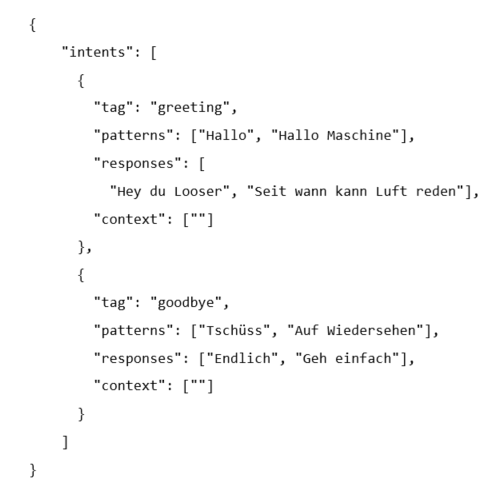
\includegraphics[width=0.8\textwidth]{Bilder_Implementierung/json_patterns.png}}
    \caption{\label{figure:Json_Patterns}Patterns Datei}
\end{figure}
\noindent
Das json-Modul wird verwendet, um die Datei zu laden und als Variable zu speichern.\\
\lstinputlisting[language=python, style=algoBericht, label={save_patterns}, basicstyle=\tiny\sffamily, captionpos=b, caption={Speichern der Patterns}]{./Listings/save_patterns.py}
Listing \ref{save_patterns} zeigt, dassine verschachtelte for-Schleife alle bereits tokenisierte Wörter in \glqq{}patterns\grqq{} extrahiert und sie der \glqq{}words\_for\_pattern\grqq{} Variable hinzufügt.
Anschließend werden jedes Paar von Mustern mit dem entsprechenden Tag einer Dokumentenliste hinzugefügt. 
Auch die Tags werden in eine Klassenliste (\glqq{}model\_classes\grqq{}) aufgenommen.
Als Nächstes wird die Wortliste genommen und alle Wörter darin lemmatisiert und kleingeschrieben. 
Nach der Sortierung der Liste sind die Daten für das Training eines Deep Learning Modells vorbereitet.\\
\lstinputlisting[language=python, style=algoBericht, label={training_test_data}, basicstyle=\tiny\sffamily, captionpos=b, caption={Initialisierung der Test- und Trainingdata}]{./Listings/training_test_data.py}
Wie in Listing \ref{training_test_data} gezeigt wird, werden zunächst die Trainingsdaten mit einer Variable \glqq{}training\grqq{} initialisiert. 
Es wird eine verschachtelte Liste erstellt, die \ac{BOW} für jedes einzelne Dokument enthält. 
Das Merkmal output\_row dient einfach als Schlüssel für die Liste. 
Dann werden die Trainingsmengen gemischt und in Training und Test aufgeteilt, wobei die Patterns die Variable X und die Intents die Variable Y sind. 
Da die Trainings- und Testdaten fertig sind, wird jetzt ein Deep-Learning-Modell von Keras namens Sequential verwendet.\\
\lstinputlisting[language=python, style=algoBericht, label={train_model}, basicstyle=\tiny\sffamily, captionpos=b, caption={Training des Modells}]{./Listings/train_model.py}
Listing \ref{speech_rec_2} zeigt, dass in diesem Fall ein \ac{MLP}-Modell verwendet wird, um das Problem der Mehrklassenklassifizierung zu lösen. 
\ac{MLP} ist eine der häufigsten Arten von neuronalen Netzen, die aus mehreren Schichten bestehen, die jeweils mehrere miteinander verbundene Neuronen enthalten. 
In der Regel werden mehrere versteckte Schichten zwischen der Eingabe- und der Ausgabeschicht verwendet, damit das Modell komplexere Merkmale aus den Eingabedaten extrahieren und die Qualität der Klassifizierung verbessern kann. 
In diesem Fall besteht das Modell aus drei Schichten: Die erste Schicht enthält 128 Neuronen, die zweite Schicht 64 Neuronen und die dritte Schicht (Ausgabeschicht) enthält die Anzahl der Neuronen, die der Anzahl der Klassen (Absichten) entspricht. 
Für die Aktivierung der Neuronen in den ersten beiden versteckten Schichten wird die Aktivierungsfunktion ReLU (Rectified Linear Unit) verwendet, für die Aktivierung der Neuronen in der Ausgabeschicht wird die Funktion Softmax verwendet, um die Zugehörigkeitswahrscheinlichkeiten der Eingabebeispiele zu jeder Klasse zu erhalten.\\\\
Als Verlustfunktion wird kategoriale Kreuzentropie (categorical\_crossentropy) verwendet, die Standardverlustfunktion für Mehrklassen-Klassifizierungsaufgaben in Keras. 
Der Optimierer, der zum Trainieren des Modells verwendet wird, ist der stochastische Gradientenabstieg mit beschleunigtem Nesterov-Gradienten (SGD mit beschleunigtem Nesterov-Gradienten), der ein schnelleres Lernen und eine höhere Genauigkeit bei Klassifizierungsaufgaben ermöglicht.\\\\
Nachdem das Modell trainiert wurde, wird das Ganze in ein Numpy-Array umgewandelt und als dialog\_model.h5 gespeichert und kann für den Dialog mit der Getränkemischmaschine verwendet werden.
\subsection{Implementierung des Dialogsystems}
\subsection{Implementierung der Bafehlverarbeitung}
\section{Implementierung der Sprachsteuerung}
Im Folgenden wird erläutert, wie die Sprachsteuerung für die Getränkemischmaschine implementiert wurde und welche Technologien dafür zum Einsatz kamen. Dabei wird zunächst auf die Spracherkennung d.h., die Umwandlung der Audiosignale (Sprachbefehl des Benutzers) in eine Form, die innerhalb des Quelltextes weiterverarbeitet werden kann, eingegangen (s. Abschnitt \ref{section:Spracherkennung}). Danach wird die Anbindung des Sprachverarbeitungssystems beschrieben, dessen Implementierung in Abschnitt \ref{section:Implementierung_Sprachverarbeitung} erklärt wird. Abschließend wird die Kommunikation mit der Mischmaschine über den Arduino illustriert (s. Abschnitt \ref{section:Befehlsverarbeitung}).
\subsection{Spracherkennung}\label{section:Spracherkennung}
Die Spracherkennung ist der erste Schritt bei der Implementierung einer Sprachsteuerung für die Getränkemischmaschine. Mit Spracherkennung ist die Aufnahme eines Tonsignals über ein Audio-Eingabegerät (Mikrofon) und die Umwandlung der Audiodaten in Text gemeint. Der Quelltext zur Implementierung der Sprachsteuerung erfolgt mit der Programmiersprache \textit{Python}, da hier sehr viele, leicht zu bedienende Bibliotheken zur Spracherkennung, -verarbeitung und \ac{KI} zur Verfügung stehen.\\\\
Für dieses Projekt viel die Wahl auf das Paket \textit{SpeechRecognition}, das die Verwendung verschiedener Spracherkennungsdienste über eine einheitliche Schnittstelle ermöglicht und zu diesem Zweck auch zur Aufnahme und Verarbeitung der Audiosignale verwendet werden kann \cite{speechrecognition}. Ein großer Vorteil davon ist, dass dadurch ein schneller Wechsel der eingesetzten \ac{API} erfolgen kann, sollte dies erforderlich sein. Die Verwendung des \textit{SpeechRecognition}-Pakets findet fast ausschließlich über die \textit{Recognizer}-Klasse statt. Um Audiosignale über eine physische Audioquelle (bspw. ein Mikrofon am Computer) aufzunehmen kann die \textit{Microphone}-Klasse verwendet werden, die ebenfalls im Paket enthalten ist. Mit Hilfe eines Objekts vom Typ \textit{Microphone} und der Methode \textit{listen} der \textit{Recognizer}-Klasse können anschließend Audiodaten aufgenommen werden, die in einem Objekt vom Typ \textit{AudioData} gespeichert sind. Die Verwendung von \textit{Recognizer} und \textit{Microphone} sind in Listing \ref{speech_rec_1} zu sehen. 
\lstinputlisting[language=python, style=algoBericht, label={speech_rec_1}, basicstyle=\tiny\sffamily, captionpos=b, caption={Audioaufnahme mit \textit{SpeechRecognition}}]{./Listings/speech_rec_1.py}
Das \textit{AudioData}-Objekt kann nun verwendet werden um die darin gespeicherten Audiodaten zu erkennen und in Text umzuwandeln. Das \textit{SpeechRecognition}-Paket stellt dafür verschiedene Möglichkeiten zur Verfügung, wie eingangs erwähnt wurde. Diese sollen im Folgenden kurz beschrieben werden:
\begin{itemize}
    \item Whisper: Whisper ist ein neuronales Netz das von der Firma \textit{OpenAI} trainiert und als Open-Source-Projekt zur Verfügung gestellt wird \cite{openai,whisper}. Neben der Fähigkeit Sprache in Text zu konvertieren kann es auch eingesetzt werden um Transkripte zu generieren, die gesprochene Sprache automatisch zu erkennen oder in die englische Sprache zu übersetzen. Das Paket \textit{SpeechRecognition} lässt sowohl die Verwendung der von \textit{OpenAI} zur Verfügung gestellten Online-\ac{API} zu, als auch die lokale Ausführung des Sprachmodells. Aufgrund der Anforderung nach Offline-Funktionalität entfällt die erste Möglichkeit (s. Kapitel \ref{chap:Anforderungen}).
    \item Sphinx: Das \textit{CMUSphinx} Projekt wird von der \ac{CMU} unterhalten und stellt eine Reihe von Werkzeugen und Bibliotheken zur Spracherkennung zur Verfügung \cite{sphinx_about}. Darunter fallen bspw. \textit{PocketSphinx}, \textit{SphinxTrain} und \textit{sphinx4}. Bei \textit{PocketSphinx} handelt es sich um eine C-Bibliothek zur Spracherkennung, die auch innerhalb von Python verwendet werden kann. \textit{SphinxTrain} hingegen stellt Ressourcen zum Trainieren eigener Modelle bereit. \textit{sphinx4} ist das Java-Equivalent zu \textit{PocketSphinx}. Somit ist für dieses Projekt nur \textit{PocketSphinx} interessant. Leider unterstützt enthält das Paket standardmäßig nur ein Modell für die englische Sprache. Anderssprachige Modelle und weitere dazugehörige Ressourcen müssen mühsam aus externen Quellen bezogen und eingebunden werden.
    \item Snowboy: \textit{Snowboy Hotword Detection} ist ein quelloffenes Projekt welches Bibliotheken für verschiedene Programmiersprachen bereitstellt, die dem Erkennen sog. \glqq{}hot words\grqq{} dienen \cite{snowboy}. Ein \textit{hot word} sind ein oder mehrere Wörter die der Aktivierung eines Sprachsteuerungssystems dienen. Bekannte Beispiele hierfür sind \glqq{}Alexa\grqq{} oder \glqq{}OK Google\grqq{}. Das System \glqq{}hört\grqq{} im Hintergrund und wartet darauf, dass das \textit{hot word} genannt wird. Anschließend nimmt das System weitere Sätze, die vom Benutzer gesprochen werden, wahr und verarbeitet diese. Ein \textit{hot word} ist notwendig damit das System nicht dauerhaft versucht Sätze zu verarbeiten, die nicht für das System gedacht sind und damit wiederholt Fehler bekommt oder unerwünschtes Verhalten an den Tag legt. Da die Ansprüche des vorliegenden Projekts an die Detektion von \textit{hot words} nicht besonders hoch sind und um die von Snowboy benötigte Rechenzeit einzusparen wird \textit{Snowboy} in diesem Projekt keine Relevanz haben. Auf die konkrete Umsetzung des \textit{hot word} Mechanismus wird später noch eingegangen. Ein weiterer Grund dafür, dass Snowboy nicht zum Einsatz kommen soll ist, dass das Projekt bereits im Jahr 2020 offiziell eingestellt wurde und nur noch von der Community weiter betrieben wird. 
    \item Vosk: Das \textit{Vosk Speech Recognition Toolkit} ist neben \textit{Whisper} und \textit{Sphinx} die dritte und letzte verfügbare offline \ac{API} für die \textit{SpeechRecognition} eine Schnittstelle bereitstellt \cite{vosk,vosk_repo}. Es wird von der \textit{Alpha Cephei Incorporation} vertrieben. Ähnlich wie bei Whisper sind vortrainierte Modelle in vielen verschiedenen Sprachen bereits vorhanden, müssen allerdings manuell heruntergeladen und dem \textit{SpeechRecognition} Paket zur Verfügung gestellt werden.
    \item Google: \textit{SpeechRecognition} bietet zwei Möglichkeiten Google-Dienste zur Konvertierung von Sprache zu Text zu verwenden. Die erste Möglichkeit besteht in der Verwendung der \textit{Google Speech API} in der \textit{Google Cloud} \cite{google_cloud_speech}. Die zweite Möglichkeit besteht in der Verwendung der \textit{Google Speech API} ohne die \textit{Google Cloud}. Die Verwendung der Google-Schnittstelle entfällt jedoch für dieses Projekt, da eine aktive Internetverbindung Voraussetzung dafür ist. Außerdem sind die Google-Dienste weder kostenfrei noch open-source.
    \item Microsoft: Auch hier gibt es zwei verschiedene Möglichkeiten Microsoft-Dienste zur Umwandlung von Sprache zu Text über das \textit{SpeechRecognition}-Paket zu nutzen. Eine davon ist die Verwendung der \textit{Speech to text} Funktion in der \textit{Microsoft Azure Cloud} \cite{azure_speech_to_text}. Hierfür sind ein aktiver \textit{Azure}-Account sowie ein gültiger \ac{API}-Schlüssel notwendig. Die zweite Möglichkeit besteht in der \textit{Microsoft Bing Voice Recognition}. Diese ist jedoch veraltet und wird nicht mehr unterstützt. Auch diese Schnittstelle enfällt jedoch wegen der notwendigen Internetverbindung und Bezahlung. 
    \item IBM: Auch die Firma IBM bietet ihre eigene Schnittstelle zur Spracherkennung mit Hilfe der von IBM entwickelten \ac{KI} \textit{Watson} an \cite{ibm_speech_to_text}. Auch hier gilt: zur Verwendung der \ac{API} ist sowohl eine aktive Internetverbindung als auch Bezahlung vorgesehen, weshalb diese Schnittstelle für das Projekt nicht in Frage kommt.
    \item Weitere Schnittstellen sind \textit{Wit.ai}, \textit{Houndify} und \textit{Tensorflow} \cite{witai,houndify,tensorflow_home}. Da diese Schnittstellen allderdings ebenso eine aktive Internetverbindung voraussetzen und damit ausscheiden soll nicht weiter auf sie eingegangen werden.
\end{itemize}
Die einzelnen \ac{API}s lassen sich jeweils über einen Methodenaufruf der Form \textit{Recognizer.recognize\_x} verwenden, wobei das \glqq{}x\grqq{} für den Namen der jeweiligen \ac{API} steht. Für dieses Projekt viel die Wahl auf die Verwendung der \textit{Whisper}-Bibliothek von \textit{OpenAI}. Dies ist damit zu begründen, dass sie von den offline verwendbaren \ac{API}s die mit Abstand am einfachsten zu verwendende ist und gleichzeitig sehr gute Ergebnisse beim Testen damit erzielt wurden. Beispielsweise werden die Modelle für viele verschiedene Sprachen bereits von OpenAI zur Verfügung gestellt und für jedes Modell stehen weitere Ausführungen zur Verfügung die nach den eigenen Ansprüchen und vorhandenen Ressourcen ausgewählt werden können. Die verschiedenen Ausführungen sind nach der \glqq{}Größe\grqq{} des Modells unterteilt in \glqq{}tiny\grqq{}, \glqq{}base\grqq{}, \glqq{}small\grqq{}, \glqq{}medium\grqq{} und \glqq{}large\grqq{} \cite{whisper_repo}.
\lstinputlisting[language=python, style=algoBericht, label={speech_rec_2}, basicstyle=\tiny\sffamily, captionpos=b, caption={Sprache zu Text mit \textit{OpenAI Whisper}}]{./Listings/speech_rec_2.py}
Listing \ref{speech_rec_2} zeigt, wie mit Hilfe der \textit{Whisper}-\ac{API} die aufgenommenen Audiodaten zu Text verarbeitet und ausgegeben werden können. Die Sprache und die Modellgröße werden bei dem Methodenaufruf \textit{Recognizer.recognize\_whisper} angegeben. Sollte das entsprechende Modell noch nicht lokal vorliegen wird dieses bei der ersten Ausführung automatisch installiert, was einen hohen Grad an Benutzerfreundlichkeit seitens der \ac{API} bedeutet. Natürlich ist es unzureichend einmal die Sprache des Benutzers aufzunehmen und in Text zu konvertieren. Insgesamt muss das Programm während des Betriebs der Getränkemischmaschine in einer Dauerschleife ausgeführt werden und der Benutzer muss die Möglichkeit haben mehrere Befehle nacheinander über die Sprachsteuerung auszuführen. Listing \ref{speech_rec_4} zeigt wie dies konkret erreicht wurde.
\lstinputlisting[language=python, style=algoBericht, label={speech_rec_4}, basicstyle=\tiny\sffamily, captionpos=b, caption={Hot-Word-Erkennung}, escapeinside={\#*}{*)}]{./Listings/speech_rec_4.py} 
Der Code der für die Konvertierung in Sprache zu Text zuständig wird nun innerhalb einer While-True-Schleife ausgeführt. Um zu verhindern, dass die Mischmaschine Befehle verarbeitet, die keine sind, soll das \textit{hot word} \glqq{}Mischmaschine\grqq{} zur Aktivierung genutzt werden. Deshalb wird in Zeile \ref{code:hot_word} nun geprüft, ob der erkannte Text mit diesem Wort beginnt und nur dann werden weitere Schritte zur Befehlsverarbeitung eingeleitet (mehr dazu in Abschnitt \ref{section:Befehlsverarbeitung}). Da davon auszugehen ist, dass die Mischmaschine an Orten eingesetzt wird, die vielen Umgebungsgeräuschen ausgesetzt sind wird in Zeile sechs außerdem die Methode \textit{speech\_recognition.Recognizer().adjust\_for\_ambient\_noise(source)} aufgerufen, die dafür sorgt, dass die Empfindlichkeit des Mikrofons automatisch an die Lautstärke der Umgebungsgeräusche angepasst wird.
\subsubsection{Herausforderungen bei der Implementierung der Spracherkennung}
Die Verwendung von \textit{Whisper} setzt die Installation von \textit{PyTorch} voraus - einem quelloffenen \ac{ML}-Framework \cite{pytorch}. Die Installation von \textit{PyTorch} kann auf zwei unterschiedlichen Wegen erfolgen:
\begin{enumerate}
    \item Unter der Benutzung vorkompilierter Distributionen mit Hilfe eines Paketverwaltungssystems wie etwa \textit{pip} \cite{pip}.
    \item Durch das eigenständige Bauen des Quelltextes auf dem lokalen Rechner.
\end{enumerate}
Da es sich bei \textit{PyTorch} um ein überaus großes und komplexes Projekt handelt ist es empfehlenswert die erste Methode anzuwenden, da der Build-Vorgang bei Methode zwei sehr viele Ressourcen benötigt.\\\\
Nach der Verwendung von \textit{pip} zur Installation von \textit{PyTorch} auf dem für das Projekt verwendeten \textit{Raspberry Pi 4B} kam es jedoch zu einem unerwarteten Fehler. Das Importieren der \textit{PyTorch}-Bibliothek ließ das Programm sofort beenden und die Nachricht \glqq{}Illegal Instruction\grqq{} auf dem Bildschirm ausgeben. Die Fehlermeldung lässt darauf schließen, dass die Bibliothek einen für den Prozessortyp unbekannten Befehl ausüben will. Drei Lösungsansätze wurden daraufhin konzipiert:
\begin{enumerate}
    \item Das Programm sollte mit einer anderen Python-Version ausgeführt werden.
    \item Das vorkompilierte Paket, das automatisch von \textit{pip} ausgewählt wurde scheint nicht auf die vorhandene Prozessorarchitektur zu passen und führt unbekannte Maschinenbefehle aus. Deshalb sollte die \textit{PyTorch}-Bibliothek selbstständig, lokal kompiliert werden.
    \item Ein anderes vorkompiliertes Paket herunterladen und installieren, das auf die vorhandene Prozessorarchitektur angepasst und optimiert ist.
    \item Sollten alle zuvor genannten Versuche scheitern muss \textit{Whisper} durch eine andere Bibliothek ersetzt werden, die keine Abhängigkeit zu \textit{PyTorch} aufweist.
\end{enumerate}
Lösungsansatz eins erwies sich als nicht effektiv. Das Programm verursachte immernoch den selben Fehler. Lösungsansatz zwei scheiterte, da der Build-Prozess mehr als den zur Verfügung stehenden \ac{RAM} des Raspberry Pi aufbrauchte. Sogar mit vier \ac{GB} zusätzlich konfiguriertem Swap-Speicher wurde der Build-Prozess nach einiger Zeit vom Betriebssystem beendet aufgrund des hohen \ac{RAM}-Verbrauchs. Lösungsansatz drei funktionierte schließlich. Mit Hilfe des vorkompilierten Pakets aus \cite{q-engineering_install_nodate} konnte \textit{PyTorch} installiert und erfolgreich importiert und verwendet werden.\\\\
Ein weiteres Problem trat bei der Verwendung des Mikrofons über die \textit{SpeechRecognition}-Bibliothek auf. Bei den Aufrufen \textit{speech\_recognition.Microphone()} und\\ \textit{speech\_recognition.Recognizer().listen(source)} kommt es auf dem Raspberry Pi zu unerwarteten Fehlermeldungen, die in Abbildung \ref{img:alsa_errors} zu sehen sind.
\begin{figure}[H]
    \centering
    \fbox{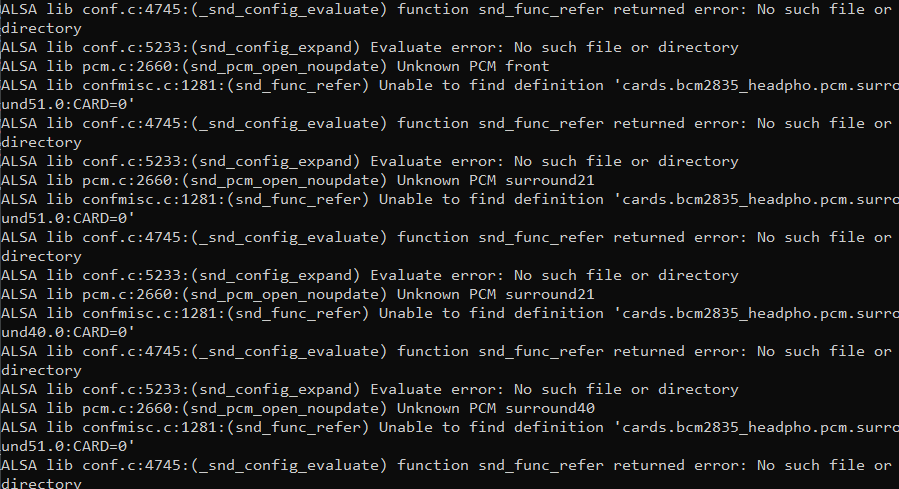
\includegraphics[width=0.8\textwidth]{./img/Bilder_Implementierung/alsa_errors.png}}
    \caption{Fehlermeldungen beim Zugriff auf das Mikrofon}
    \label{img:alsa_errors}
\end{figure}
\noindent
Zwar kann das Programm trotz der Meldungen fehlerfrei ausgeführt werden, jedoch stören die Meldungen bspw. beim Debuggen und irritieren evtl. Programmierer, die zu einem späteren Zeitpunkt einen Blick auf das Projekt werfen. Um die Fehlermeldungen zu umgehen wurde deshalb im finalen Quelltext die Fehlerbehandlungsfunktion der \textit{libasound}-Bibliothek ausgetauscht wie in Listing \ref{speech_rec_3} zu sehen ist.
\lstinputlisting[language=python, style=algoBericht, label={speech_rec_3}, basicstyle=\tiny\sffamily, captionpos=b, caption={Fehlerbehandlung}, escapeinside={\#*}{*)}]{./Listings/speech_rec_3.py}
Für einen Vorher-/Nachher-Vergleich sei auf Listing \ref{speech_rec_2} verwiesen. Die Zeilen \ref{code:error_handler_begin} bis \ref{code:error_handler_end} dienen der Definition einer C-Funktion zur Fehlerbehandlung, die bei ihrer Ausführung die auftretende Meldung ignoriert. In Zeile \ref{code:set_handler} wird die Standard Fehlerfunktion durch diese ersetzt und in Zeile \ref{code:set_default_handler} wieder zurückgeändert. 
\subsection{Befehlsverarbeitung in der Mischmaschine}\label{section:Befehlsverarbeitung}
Nachdem die Sprache des Benutzers erkannt, in Text konvertiert und durch das Sprachmodell interpretiert wurde muss der zurückerhaltene Befehl vom Raspberry Pi and den Arduino in der Getränkemischmaschine gesendet werden. Zur Umsetzung der Kommunikation zwischen Raspberry Pi und Arduino kommt die \textit{PySerial}-Bibliothek zum Einsatz \cite{pyserial}. Listing \ref{serial_1_py} zeigt, wie die Bibliothek zum Versenden von Nachrichten an ein Gerät über die serielle Schnittstelle erfolgen kann.
\lstinputlisting[language=python, style=algoBericht, label={serial_1_py}, basicstyle=\tiny\sffamily, captionpos=b, caption={Serielle Kommunikation in Python}, escapeinside={\#*}{*)}]{./Listings/serial_1.py}
Das Programm öffnet in Zeile \ref{code:open_serial} die serielle Schnittstelle zu dem Gerät mit dem Namen \glqq{}ttyACM0\grqq{}, mit einer Baud-Rate von 9600 und einem Timeout von fünf Sekunden. Der Gerätename ist je nach Gerät und Betriebssystem unterschiedlich und muss zuvor mit den verfügbaren Betriebssystemmitteln bestimmt werden. Die Baud-Rate gibt an, mit welcher Geschwindigkeit Symbole über die Schnittstelle gesendet werden. Die Baud-Rate muss sowohl beim Sender als auch beim Empfänger gleich sein, da es sonst zu Kommunikationsproblemen kommt. Der Timeout steuert wie lange bei einer Leseoperation gewartet werden soll, bis alle zu lesenden Bytes im Puffer vorhanden sind.\\\\
In der darauffolgenden Zeile wird der Eingabepuffer geleert, um zu verhindern, dass unvollständige Daten an den Empfänger gesendet werden, die beim letzten Programmdurchlauf im Puffer verblieben sein könnten. Da der Verbindungsaufbau mit dem Gerät einige Zeit dauern kann wird die Programmausührung in Zeile \ref{code:sleep_serial} zunächst um fünf Sekunden verzögert. Das nachfolgende Programm sendet in einer While-True-Schleife mehrere Nachrichten über die serielle Schnittstelle, die über einen Zähler voneinander zu unterscheiden sind. Anschließend wird in Zeile zehn eine Nachricht zurück erwartet die anschließend auf der Kommandozeile ausgegeben wird.\\\\
In Listing \ref{serial_1_ino} ist der Quelltext auf Empfängerseite zu sehen, der dafür zuständig ist die in Listing \ref{serial_1_py} generierten Nachrichten zu empfangen und Daten zurückzusenden.
\lstinputlisting[language=c++, style=algoBericht, label={serial_1_ino}, basicstyle=\tiny\sffamily, captionpos=b, caption={Serielle Kommunikation in Python}]{./Listings/serial_1.ino}
Das Programm ist in der Arduino-Programmiersprache verfasst und besteht, wie vorgegeben, aus einer \textit{setup} und einer \textit{loop} Methode. Die \textit{setup} Methode wird einmalig beim Start des Programms, wenn der Arduino mit Strom versorgt wird, ausgeführt wohingegen die \textit{loop} Methode dauerhaft während der Arduino mit Strom versorgt ist wiederholt ausgeführt wird. In der \textit{setup}-Methode wird die serielle Schnittstelle mit einer Baud-Rate von 9600 geöffnet. Innerhalb der \textit{loop}-Methode wird geprüft, ob Bytes in den Eingabepuffer geschrieben wurden. Ist dies der Fall wird der If-Block betreten und die in den Puffer geschriebenen Bytes werden bis zu einem vorgegebenen Terminalsymbol (in diesem Fall ein Zeilenumbruch) eingelesen und in ein String-Objekt konvertiert. Mit dem Aufruf \textit{Serial.println(data)} wird der empfangene String über die serielle Schnittstelle zurück an den ursprünglichen Sender übertragen. Dabei handelt es sich um den String, der in dem Programm aus Listing \ref{serial_1_py} in Zeile \ref{code:read_serial} erwartet wird.\\\\
Die eben an einem einfachen Beispiel beschriebene Vorgehensweise/Implementierung kann eins zu eins auf die Problemstellung des vorliegenden Projekts übertragen werden. Statt der generischen Nachricht wird das Kommando, das von dem Sprachmodell zurückgegeben wird übertragen. Auf Seiten des Arduinos muss das Kommando interpretiert und die entsprechenden Aktionen innerhalb der Mischmaschine ausgelöst werden. Listing \ref{serial_2_py} zeigt wie auf seiten des Raspberry Pi die eben beschriebenen Techniken in das Hauptprogramm aus Listing \ref{speech_rec_3} integriert werden können. Die Definition und das Setzen der C-Fehlerbehandlungsfunktion wurde aus Gründen der Übersichtlichkeit weggelassen.
\lstinputlisting[language=python, style=algoBericht, label={serial_2_py}, basicstyle=\tiny\sffamily, captionpos=b, caption={Serielle Kommunikation für die Mischmaschine}, escapeinside={\#*}{*)}]{./Listings/serial_2.py}
In den Zeilen \ref{code:begin_model_stub} und \ref{code:end_model_stub} wird eine Methode definiert, die das Sprachmodell, welches die Sprache des Benutzers interpretiert und einen Maschinenbefehl und eine Antwort zurückgibt, nachahmen soll. Das Kommando besteht aus vier natürlichen Zahlen, die die Prozentwerte der jeweiligen Behälter in der Mischmaschine darstellen. Der String \glqq{}50,50,0,0\grqq{} ist also so zu interpretieren, dass das Mischungsverhältnis zu 50 Prozent aus Behälter eins und zu 50 Prozent aus Behälter zwei bestehen soll. In Zeile \ref{code:send_command} wird dieses Kommando an den Arduino, welcher die Mischmaschine steuert, übertragen. Listing \ref{serial_2_ino} zeigt einen Ausschnitt des abgeänderten Code auf Seiten des Arduinos. Der gesamte Quelltext ist in Anhang \ref{Anhang_A} zu finden.
\lstinputlisting[language=c++, style=algoBericht, label={serial_2_ino}, basicstyle=\tiny\sffamily, captionpos=b, caption={Interpretation der Kommandos}]{./Listings/serial_2.ino}
Mit der Methode \textit{getValueAt(String, int): int} wird die Prozentangabe an der gewünschten Stelle im Kommandostring ausgelesen. In der Hauptprogrammschleife werden die Pumpen eins bis vier mit ihren entsprechenden Werten angesprochen. Das Delay in der letzten Zeile des If-Blocks sorgt dafür, dass die Pumpen nicht sofort wieder in der nächsten Schleifeniteration ausgeschaltet werden.
\subsubsection{Herausforderungen bei der Implementierung der Befehlsverarbeitung}
Eine Herasuforderung bestand in der Steuerung der seriellen Kommunikation von Raspberry Pi und Touch-Display mit dem Arduino. Zunächst wurde versehentlich die selbe serielle Schnittstelle sowohl für das \textit{Nextion}-Display als auch den Raspberry Pi verwendet. Dies führte dazu, dass der Empfänger (in diesem Fall der Arduino, welcher die Mischmaschine steuert) korrumpierte Daten erhielt. Die korrumpierten Daten waren für den Arduino nicht mehr lesbar, sodass die Mischmaschine auf keine Benutezreingaben mehr reagieren konnte. Die anfängliche Verwirrung entstand dadurch, dass das \textit{Serial}-Objekt sich auf die Standardschnittstelle bezieht, welche sowohl den USB-Hub, als auch die TX0/RX0-Pins mit einschließt, an die das Display ursprünglich angeschlossen war. Die verfügbaren Pins sind in Abbildung \ref{fig:pinout_mega} zu sehen \cite{arduino_mega}.
\begin{figure}[H]
    \centering
    \fbox{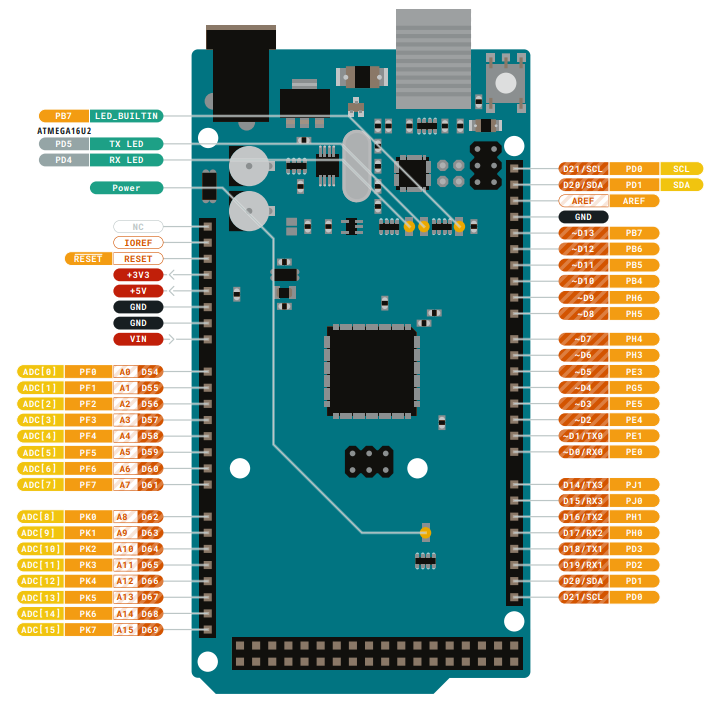
\includegraphics[width=0.8\textwidth]{./img/Bilder_Implementierung/pinout_mega.png}}
    \caption{Pinout für Arduino Mega}
    \label{fig:pinout_mega}
\end{figure}
\noindent
Nachdem die Ursache des Problems gefunden wurde konnte nach einer Lösung gesucht werden. Die Lösung bestand darin, das \textit{Nextion}-Display über eine andere serielle Schnittstelle mit dem Ardunino kommunizieren zu lassen. Zu diesem Zweck wurde das \textit{Serial2}-Objekt gewählt welches sich auf die beiden Pins 16 und 17 bezieht. Anhang \ref{Anhang_A}, Zeile \ref{code:serial2} zeigt, wie über die \textit{Serial2}-Schnittstelle die Kommunikation mit dem \textit{Nextion}-Display initialisiert wird, wohingegen der Raspberry Pi weiterhin den USB-Hub und damit die Standardschnittstelle benutzt. So konnte die gleichzeitige Kommunikation zweier Geräte mit dem Arduino gewährleistet werden.\\\\
Eine weitere Herausforderung bestand in einem Programmierfehler, der dazu führte, dass die Mischmaschine nicht wie gewünscht über die Sprachsteuerung bedient werden konnte. Der Fehler war auf eine falsche Verwendung der \textit{PySerial}-Bibliothek zurückzuführen. In einer früheren Version des Programms aus Listing \ref{serial_2_py} wurde der Funktionsaufruf \textit{serial.Serial(name, rate, timeout).reset\_input\_buffer()}, der in Zeile \ref{code:open_serial_serial_2} zu sehen ist, in jeder Schleifeniteration der While-True-Schleife ausgeführt. Die Idee hierbei war, dass vor jeder neuen Übertragung der Eingabepuffer geleert werden muss, da evtl. korrupte Daten darin vorliegen. Dabei handelt es sich allerdings um einen Irrtum, da in jeder Schleifeniteration alle Bytes zum Arduino gesendet und alle Bytes vom Arduino zurückerhalten werden. Der einzige Fall in dem es möglich ist, dass korrupte Daten in dem Eingabepuffer zurückgeblieben sind ist, wenn das Programm unerwartet stoppt, bspw. wenn der Benutzer einen Stopp veranlasst oder die Stromversorgung abbricht. Deshalb darf der Eingabepuffer nur am Anfang des Programms einmal geleert werden und nicht in jeder Schleifeniteration, da sonst die Nutzdaten, die tatsächlich übertragen werden sollen, aus dem Puffer entfernt werden.
\subsection{Sprachausgabe} 
Die Sprachausgabe beschäftigt sich damit, die Antwort, die von dem Sprachmodell in textform ausgegeben wird, durch Lautsprecher in der Mischmaschine auszugeben und sie somit Teilnehmer einer Konversation mit dem Benutzer werden zu lassen. Um dies zu bewerkstelligen kommt die \textit{pyttsx3}-Bibliothek zum Einsatz \cite{pyttsx3}. Listing \ref{tts_1} zeigt die Benutzung der Bibliothek anhand eines einfachen Beispiels.
\lstinputlisting[language=python, style=algoBericht, label={tts_1}, basicstyle=\tiny\sffamily, captionpos=b, caption={Text-to-Speech mit \textit{pyttsx3}}, escapeinside={\#*}{*)}]{./Listings/tts_1.py}
Zunächst wird ein Objekt vom Typ \textit{pyttsx3.Engine} durch den Aufruf \textit{pyttsx3.init()} erzeugt. Dabei werden automatisch die vorhandenen Treiber auf dem Gerät gesucht, die für die Sprachausgabe verwendet werden können. Die am häufigsten vorkommenden Treiber sind \textit{SAPI5} für Windows, \textit{NSSpeechSynthesizer} für Mac OS X und \textit{eSpeak} für die sonstigen Betriebssysteme wie etwa Raspberry Pi OS. Die Treiber stellen verschiedene \glqq{}Stimmen\grqq{} zur Verfügung, die in der Property \textit{voices} gespeichert werden und wie in Zeile \ref{code:get_voices} zu sehen ist mit einem Aufruf von \textit{Engine.getProperty(\glqq{}voices\grqq{})} abgerufen werden können. In diesem Beispiel wird die von \textit{pyttsx3} zu verwendende Stimme auf die Stimme an Index eins gesetzt. Wenn eine bestimmte Stimme gewünscht ist, dann müssen die von \textit{pyttsx3} gefundenen Stimmen auf ihre Attribute/Eigenschaften hin untersucht werden. Ein Objekt vom Typ \textit{pyttsx3.voice.Voice} speichert das Alter, Geschlecht, die unterstützten Sprachen und den Namen als auch eine eindeutige Kennung der Stimme. Somit kann entschieden werden, welche Stimme am besten für den eigenen Anwendungsfall geeignet ist. Alternativ kann ein eigener Treiber/Synthesizer implementiert werden. Für die schlussendliche Implementierung der Sprachausgabe innerhalb des Hauptprogramms sei auf Anhang \ref{Anhang_B} verwiesen.
\subsection{Anbindung des Sprachmodells an die Mischmaschine}
Die Anbindung des Sprachmodells and die Mischmaschine war schlussendlich ohne großen Aufwand möglich. Es musste lediglich der Platzhalter aus Listing \ref{serial_2_py} in den Zeilen \ref{code:begin_model_stub} und \ref{code:end_model_stub} durch einen Methodenaufruf der tatsächlichen Implementierung in Zeile \ref{code:real_model} ersetzt werden, wie im Anhang \ref{Anhang_B} zu sehen ist. Für den vollständigen Code des Sprachmodells sei auf \ref{Anhang_C} verwiesen.   
\endinput


